\subsection{Future Graph Decompositions}
\label{sec:future-graphs}

The three dependency graphs defined above---$G_{\mathrm{module}}$, $G_{\mathrm{thm}}$, and $G_{\mathrm{ns}}^{(k)}$---are constructed from data available through the current extraction pipeline (\texttt{importGraph}, \texttt{lean4export}, \texttt{lean-training-data}). In this section, we define five additional graph decompositions that require deeper access to Lean's elaboration layer, specifically the ability to inspect type signatures vs.\ proof terms, trace typeclass instance synthesis, and read declaration-level metadata. We include these definitions to establish a formal framework for future empirical work; the analyses themselves are deferred pending access to metaprogramming-level extraction tools. \xinze{Hi Adam! Could you help us use LeanScout to extract the data types defined in the following subsections (statement vs proof deps, typeclass instance edges, public/private import flags, declaration attributes, etc.)? That would let us turn these formal definitions into actual empirical results. Thanks!}

Throughout, we use the following notation. The \emph{Lean environment}~$\mathcal{E}$ denotes the compiled state of \module{Mathlib} at commit \texttt{534cf0b}. Each declaration~$d \in \mathcal{D}$ consists of a type~$d.\tau$ (the statement or signature) and, for non-axiomatic declarations, a value~$d.\pi$ (the proof term or definition body). We write $\mathrm{refs}(e)$ for the set of all named constants referenced in an expression~$e$.

\subsubsection{The Statement and Proof Dependency Graphs}
\label{sec:stmt-proof-graph}

The declaration graph $G_{\mathrm{thm}}$ (Definition~\ref{def:thm-graph}) aggregates all premise references without distinguishing \emph{where} in a declaration each reference occurs. A finer decomposition separates the dependencies required by a declaration's \emph{statement} from those required only by its \emph{proof}.

\begin{definition}[Statement and proof dependency]\label{def:stmt-proof-dep}
For declarations $a, b \in \mathcal{D}$, define:
\begin{align*}
  a \xrightarrow{S} b &\iff b \in \mathrm{refs}(a.\tau), \\
  a \xrightarrow{P} b &\iff b \in \mathrm{refs}(a.\pi) \setminus \mathrm{refs}(a.\tau).
\end{align*}
The \emph{statement dependency graph} is $G_S = (\mathcal{D}, E_S)$ where $E_S = \{(a,b) : a \xrightarrow{S} b\}$, and the \emph{pure proof dependency graph} is $G_P = (\mathcal{D}, E_P)$ where $E_P = \{(a,b) : a \xrightarrow{P} b\}$. An edge $(a,b) \in E_{\mathrm{thm}}$ that belongs to both $\mathrm{refs}(a.\tau)$ and $\mathrm{refs}(a.\pi)$ is classified as a \emph{mixed edge} $E_{SP}$. This yields a partition $E_{\mathrm{thm}} = E_S \sqcup E_P \sqcup E_{SP}$ (where $E_S$ excludes mixed edges for disjointness, i.e., $E_S$ consists of edges in $\mathrm{refs}(a.\tau) \setminus \mathrm{refs}(a.\pi)$, $E_{SP} = \mathrm{refs}(a.\tau) \cap \mathrm{refs}(a.\pi)$, and $E_P$ as above).
\end{definition}

\begin{figure}[!htb]
\centering
\begin{subfigure}[t]{0.52\textwidth}
\centering
\vspace{0pt}
\raggedright\scriptsize\ttfamily
\textbf{theorem} \textcolor{red!70!black}{length\_nil}\\
\hspace{1em}: [].{\textcolor{teal}{length}} = 0 := rfl\\[6pt]
\textbf{theorem} \textcolor{red!70!black}{length\_cons} (a : $\alpha$) (l : List $\alpha$)\\
\hspace{1em}: (a :: l).{\textcolor{teal}{length}} = l.{\textcolor{teal}{length}} + 1 := rfl\\[6pt]
\textbf{theorem} \textcolor{red!70!black}{length\_append} (l1 l2 : List $\alpha$)\\
\hspace{1em}: (l1 ++ l2).{\textcolor{violet}{length}} = l1.{\textcolor{violet}{length}} + l2.{\textcolor{violet}{length}}\\
\hspace{1em}:= \textbf{by} induction l1 \textbf{with}\\
\hspace{1em}| nil => simp [\textcolor{orange!80!red}{length\_nil}]\\
\hspace{1em}| cons a l ih => simp [\textcolor{orange!80!red}{length\_cons}, ih]
\caption{Source code: references colored by edge type.}
\label{fig:sp-source}
\end{subfigure}%
\hfill
\begin{subfigure}[t]{0.44\textwidth}
\centering
\vspace{0pt}
\begin{tikzpicture}[
  every node/.style={font=\scriptsize, inner sep=2pt},
  dot/.style={circle, fill=red!70!black, minimum size=3.5pt, inner sep=0pt},
  sedge/.style={->, >=Stealth, teal, semithick},
  pedge/.style={->, >=Stealth, orange!80!red, semithick, dashed},
  spedge/.style={->, >=Stealth, violet, thick},
]
  % Row 1: length_append
  \node[dot, label={[font=\tiny\ttfamily, red!70!black]above:length\_append}]
    (la) at (2, 3.2) {};
  % Row 2: length_nil, length_cons
  \node[dot, label={[font=\tiny\ttfamily, red!70!black]left:length\_nil}]
    (ln) at (0.3, 1.6) {};
  \node[dot, label={[font=\tiny\ttfamily, red!70!black]right:length\_cons}]
    (lc) at (3.7, 1.6) {};
  % Row 3: length (definition)
  \node[dot, label={[font=\tiny\ttfamily, red!70!black]below:length}]
    (ll) at (2, 0) {};
  % P edges (proof-only): orange dashed
  \draw[pedge] (la) -- (ln);
  \draw[pedge] (la) -- (lc);
  % SP edge (mixed): violet thick
  \draw[spedge] (la) -- (ll);
  % S edges (statement-only): teal solid
  \draw[sedge] (ln) -- (ll);
  \draw[sedge] (lc) -- (ll);
\end{tikzpicture}
\caption{$E_{\mathrm{thm}} = \textcolor{teal}{E_S} \sqcup \textcolor{orange!80!red}{E_P} \sqcup \textcolor{violet}{E_{SP}}$.}
\label{fig:sp-graph}
\end{subfigure}
\caption{Statement vs.\ proof decomposition (Definition~\ref{def:stmt-proof-dep}). (a)~Source code for three \texttt{List.length} theorems: \textcolor{teal}{teal} = reference only in the type~$\tau$ ($E_S$), \textcolor{orange!80!red}{orange dashed} = only in the proof~$\pi$ ($E_P$), \textcolor{violet}{violet} = in both ($E_{SP}$). For \decl{length\_nil} and \decl{length\_cons}, the definition \decl{length} appears only in~$\tau$; for \decl{length\_append}, it appears in both~$\tau$ and~$\pi$. (b)~The edge-classified subgraph. All names have the \texttt{List.}\ prefix removed.}
\label{fig:stmt-proof-decomp}
\end{figure}

This decomposition directly instantiates the paper's central distinction. The statement dependency graph~$G_S$ captures \emph{inherited mathematical structure}: what a theorem asserts depends on logically prior definitions and results that are, in principle, invariant under changes of proof strategy. The pure proof dependency graph~$G_P$ captures \emph{human organizational process}: the choice of which lemmas, tactics, and automation to invoke reflects the tools, conventions, and taste of the proving community. The ratio $\rho = |E_P| / |E_{\mathrm{thm}}|$ would directly measure how much of the observed dependency network is proof engineering rather than mathematical necessity.

\paragraph{Planned analyses.}
Compare degree distributions, DAG depth profiles, community structure, and hub identity between~$G_S$ and~$G_P$. If statement-level dependencies form a sparser, deeper graph while proof-level dependencies are denser and shallower, this would confirm that the topological inversion observed in \S\ref{sec:dag-depth} (153-layer module hierarchy vs.\ 84-layer declaration DAG) has a finer analog at the edge level.

\emph{Empirical analysis of this decomposition requires metaprogramming access to Lean's elaboration layer (specifically, separate traversal of \texttt{ConstantInfo.type} and \texttt{ConstantInfo.value}) and is deferred to future work.}

\begin{remark}[Proof-internal dependency structure]\label{rem:local-deps}
The decomposition $G_S / G_P$ refines the \emph{edges} of $G_{\mathrm{thm}}$. A complementary refinement concerns the \emph{internal structure} of each node: proof terms may contain local declarations introduced by \texttt{have}, \texttt{let}, or \texttt{suffices}, forming a proof-internal dependency tree~$G_{\mathrm{local}}(d)$ within each declaration~$d$. The size $|V(G_{\mathrm{local}}(d))|$ and depth of this tree measure proof complexity at a finer granularity than the proof term size~$\kappa(d)$ defined in \S\ref{sec:decl-metadata}. Extracting this structure requires access to the elaborated proof term or \texttt{InfoTree} and is left to future work.
\end{remark}

\subsubsection{The Typeclass Instance Graph}
\label{sec:typeclass-graph}

The hub nodes identified in \S\ref{sec:theorem-premise}---\decl{OfNat.ofNat} (in-degree $89{,}936$), \decl{DFunLike.coe} ($65{,}437$), \decl{Eq.refl} ($69{,}580$)---owe much of their centrality to Lean's typeclass instance synthesis, which automatically inserts premise references invisible to the proof author. Isolating these synthesized edges would separate the \emph{language infrastructure} layer from the \emph{mathematical content} layer identified qualitatively in Remark~\ref{rem:two-layers}.

\begin{definition}[Typeclass instance graph]\label{def:tc-graph}
Let $\mathcal{C} \subset \mathcal{D}$ be the set of all typeclass declarations and $\mathcal{I} \subset \mathcal{D}$ the set of all instance declarations. For each instance $i \in \mathcal{I}$, let $\mathrm{target}(i) \in \mathcal{C}$ be the class it provides and $\mathrm{requires}(i) \subseteq \mathcal{C}$ the classes it depends on as preconditions. The \emph{typeclass instance graph} is
\[
  G_{\mathrm{tc}} = (\mathcal{C},\, E_{\mathrm{tc}}), \quad (C_1, C_2) \in E_{\mathrm{tc}} \iff \exists\, i \in \mathcal{I} : \mathrm{target}(i) = C_2 \land C_1 \in \mathrm{requires}(i).
\]
\end{definition}

\begin{definition}[Synthesized vs.\ explicit edge partition]\label{def:synth-partition}
For each edge $(a, b) \in E_{\mathrm{thm}}$, define
\[
  \mathrm{synth}(a, b) =
  \begin{cases}
    1 & \text{if } b \text{ was inserted by typeclass instance synthesis during elaboration}, \\
    0 & \text{if } b \text{ was explicitly referenced in the source}.
  \end{cases}
\]
This partitions $E_{\mathrm{thm}} = E_{\mathrm{explicit}} \sqcup E_{\mathrm{synth}}$. The \emph{synthesis ratio} $\sigma = |E_{\mathrm{synth}}| / |E_{\mathrm{thm}}|$ measures the fraction of the observed dependency structure attributable to the proof assistant's type system rather than to mathematical logic.
\end{definition}

\begin{figure}[!htb]
\centering
\begin{subfigure}[t]{0.50\textwidth}
\centering
\vspace{0pt}
\raggedright\scriptsize\ttfamily
\textbf{theorem} \textcolor{red!70!black}{add\_zero} [AddMonoid $\alpha$] (a : $\alpha$)\\
\hspace{1em}: a + 0 = a := \textcolor{red!70!black}{AddMonoid.add\_zero} a\\[8pt]
\textnormal{\sffamily Elaborated term references:}\\[2pt]
\hspace{1em}\textcolor{red!70!black}{AddMonoid.add\_zero}%
  \textnormal{\sffamily\tiny\textcolor{gray!60}{\hspace{4pt}--- explicit}}\\
\hspace{1em}\textcolor{gray!50}{HAdd.hAdd}%
  \textnormal{\sffamily\tiny\textcolor{gray!60}{\hspace{4pt}--- synth.\ for \texttt{+}}}\\
\hspace{1em}\textcolor{gray!50}{OfNat.ofNat}%
  \textnormal{\sffamily\tiny\textcolor{gray!60}{\hspace{4pt}--- synth.\ for \texttt{0}}}
\caption{Source: only \decl{AddMonoid.add\_zero} is explicit; \texttt{+}~and~\texttt{0} trigger instance synthesis.}
\label{fig:tc-source}
\end{subfigure}%
\hfill
\begin{subfigure}[t]{0.46\textwidth}
\centering
\vspace{0pt}
\begin{tikzpicture}[
  every node/.style={font=\scriptsize, inner sep=2pt},
  dot/.style={circle, fill=red!70!black, minimum size=3.5pt, inner sep=0pt},
  sdot/.style={circle, fill=gray!50, minimum size=3.5pt, inner sep=0pt},
  elink/.style={->, >=Stealth, red!70!black, semithick},
  slink/.style={->, >=Stealth, gray!50, semithick, dashed},
]
  % Background zones (drawn first, behind nodes)
  \fill[red!6, rounded corners=3pt] (-0.6, -0.5) rectangle (1.6, 1.0);
  \node[font=\tiny\sffamily\itshape, red!40!black] at (0.5, 0.85) {math content};
  \fill[gray!8, rounded corners=3pt] (1.9, -0.5) rectangle (5.0, 1.0);
  \node[font=\tiny\sffamily\itshape, gray!50] at (3.45, 0.85) {language infrastructure};
  % Top node: the theorem
  \node[dot, label={[font=\tiny\ttfamily, red!70!black]above:add\_zero}]
    (thm) at (2.3, 2.8) {};
  % Explicit dep (math content)
  \node[dot, label={[font=\tiny\ttfamily, red!70!black]below:AddMonoid.add\_zero}]
    (axiom) at (0.5, 0.2) {};
  % Synthesized deps (language infrastructure)
  \node[sdot, label={[font=\tiny\ttfamily, gray!60]below:HAdd.hAdd}]
    (hadd) at (2.8, 0.2) {};
  \node[sdot, label={[font=\tiny\ttfamily, gray!60]below:OfNat.ofNat}]
    (ofnat) at (4.3, 0.2) {};
  % Explicit edge (solid red)
  \draw[elink] (thm) -- (axiom);
  % Synthesized edges (dashed gray)
  \draw[slink] (thm) -- (hadd);
  \draw[slink] (thm) -- (ofnat);
\end{tikzpicture}
\caption{$E_{\mathrm{thm}} = \textcolor{red!70!black}{E_{\mathrm{explicit}}} \sqcup \textcolor{gray!50}{E_{\mathrm{synth}}}$.}
\label{fig:tc-graph}
\end{subfigure}
\caption{Synthesized vs.\ explicit edge partition (Definitions~\ref{def:tc-graph},~\ref{def:synth-partition}). (a)~In the source for \decl{add\_zero}, only \decl{AddMonoid.add\_zero} is an explicit reference; the notation~\texttt{+} and literal~\texttt{0} each trigger typeclass instance synthesis, silently inserting \textcolor{gray!50}{synthesized edges}. (b)~The subgraph of $G_{\mathrm{thm}}$: \textcolor{red!70!black}{solid} = explicit, \textcolor{gray!50}{dashed} = synthesized. The two zones separate mathematical content from language infrastructure (Remark~\ref{rem:two-layers}). Hub nodes such as \decl{OfNat.ofNat} (in-degree $89{,}936$) accumulate high centrality primarily through synthesized edges.}
\label{fig:synth-partition}
\end{figure}

The typeclass system is Lean~4's mechanism for ad-hoc polymorphism---a \emph{tool-specific} organizational layer that has no analog in traditional mathematics. Baanen~\cite{baanen2022} demonstrated that typeclass design choices (bundled vs.\ unbundled) significantly reshape dependency structure; $G_{\mathrm{tc}}$ would isolate this effect. Recomputing centrality on the ``math-only'' subgraph $G_{\mathrm{thm}} \setminus E_{\mathrm{synth}}$ would test whether the hub structure shifts from language infrastructure (\decl{OfNat.ofNat}, \decl{DFunLike.coe}) to mathematical content (\decl{CategoryTheory.Category}, \decl{Real}).

\paragraph{Coercion chains.}
A complementary source of automatically inserted edges is the \emph{coercion} system. Lean allows automatic type coercions (e.g., $\mathbb{N} \hookrightarrow \mathbb{Z} \hookrightarrow \mathbb{Q}$), which the elaborator chains silently. Let $\mathcal{K} \subset \mathcal{D}$ be the set of all registered coercion instances. The \emph{coercion graph} $G_{\mathrm{coe}} = (\mathcal{T},\, E_{\mathrm{coe}})$ has types as nodes and coercion instances as edges: $(T_1, T_2) \in E_{\mathrm{coe}}$ if there exists a coercion $T_1 \to T_2$ registered in the environment. Long coercion chains (paths of length $\ge 3$ in $G_{\mathrm{coe}}$) degrade compilation performance and can produce opaque error messages; the diameter and maximum chain length of $G_{\mathrm{coe}}$ directly measure this fragility. Together, $G_{\mathrm{tc}}$ and $G_{\mathrm{coe}}$ capture the two main mechanisms by which Lean's type system silently inflates the dependency graph.

\paragraph{Planned analyses.}
Measure $\sigma$ to quantify the typeclass overhead. Recompute degree distributions and centrality rankings on $G_{\mathrm{thm}} \setminus E_{\mathrm{synth}}$. Compare community structure with and without synthesized edges. Compute the diameter and chain-length distribution of $G_{\mathrm{coe}}$.

\emph{Empirical analysis requires tracing typeclass instance synthesis and coercion resolution during elaboration and is deferred to future work.}

\subsubsection{The Visibility Graph}
\label{sec:visibility-graph}

The module graph $G_{\mathrm{module}}$ (Definition~\ref{def:module-graph}) treats all \texttt{import} edges uniformly. Since November 2025, Lean~4's module system~\cite{lean4modules} distinguishes \texttt{public import} from \texttt{import} (private), allowing modules to selectively limit transitive visibility.

\begin{definition}[Visibility graph]\label{def:visibility-graph}
For each import edge $(m_i, m_j) \in E_{\mathrm{mod}}$, let
\[
  \mathrm{vis}(m_i, m_j) \in \{\texttt{public},\, \texttt{private}\}.
\]
The \emph{public import subgraph} is
\[
  G_{\mathrm{mod}}^{\mathrm{pub}} = (\mathcal{M},\, \{(m_i, m_j) \in E_{\mathrm{mod}} : \mathrm{vis}(m_i, m_j) = \texttt{public}\}).
\]
The transitive closure of $G_{\mathrm{mod}}^{\mathrm{pub}}$ determines the actual namespace visibility scope---which declarations are transitively accessible from which modules.
\end{definition}

\begin{figure}[!htb]
\centering
\begin{subfigure}[t]{0.48\textwidth}
\centering
\vspace{0pt}
\raggedright\scriptsize\ttfamily
\textsf{\bfseries\color{blue!60!black}Data/Nat/Notation.lean}\\[2pt]
\textbf{public import} \textcolor{blue!60!black}{Init}%
\hfill\textnormal{\sffamily\tiny\textcolor{gray!60}{re-exports Init's declarations}}\\[10pt]
\textsf{\itshape\normalfont\sffamily vs.}\\[10pt]
\textsf{\bfseries\color{blue!60!black}Data/Nat/Notation.lean}\\[2pt]
\textbf{import} \textcolor{blue!60!black}{Init}%
\hfill\textnormal{\sffamily\tiny\textcolor{gray!60}{Init hidden from importers}}
\caption{\texttt{public import} re-exports; plain \texttt{import} keeps declarations private.}
\label{fig:vis-source}
\end{subfigure}%
\hfill
\begin{subfigure}[t]{0.48\textwidth}
\centering
\vspace{0pt}
\begin{tikzpicture}[
  every node/.style={font=\scriptsize, inner sep=2pt},
  dot/.style={circle, fill=blue!60!black, minimum size=4pt, inner sep=0pt},
  pub/.style={->, >=Stealth, blue!60!black, thick},
  priv/.style={->, >=Stealth, blue!60!black, thick, dashed},
]
  % Left: all public
  \node[font=\tiny\sffamily\bfseries, blue!60!black] at (0.7, 3.8)
    {$G_{\mathrm{mod}}^{\mathrm{pub}} = G_{\mathrm{mod}}$};
  \fill[blue!6, rounded corners=3pt] (-0.2, -0.3) rectangle (1.6, 3.5);
  \node[font=\tiny\sffamily\itshape, blue!40!black] at (0.7, -0.6)
    {A sees \{B, C\}};
  \node[dot, label={[font=\tiny\ttfamily, blue!60!black]right:A}]
    (a1) at (0.7, 3.0) {};
  \node[dot, label={[font=\tiny\ttfamily, blue!60!black]right:B}]
    (b1) at (0.7, 1.5) {};
  \node[dot, label={[font=\tiny\ttfamily, blue!60!black]right:C}]
    (c1) at (0.7, 0.0) {};
  \draw[pub] (a1) -- node[left, font=\tiny\sffamily, text=blue!50!black] {pub} (b1);
  \draw[pub] (b1) -- node[left, font=\tiny\sffamily, text=blue!50!black] {pub} (c1);
  % Right: private inner import
  \node[font=\tiny\sffamily\bfseries, blue!60!black] at (3.7, 3.8)
    {$G_{\mathrm{mod}}^{\mathrm{pub}} \subset G_{\mathrm{mod}}$};
  \fill[blue!6, rounded corners=3pt] (2.8, 0.9) rectangle (4.6, 3.5);
  \node[font=\tiny\sffamily\itshape, blue!40!black] at (3.7, -0.6)
    {A sees \{B\} only};
  \node[dot, label={[font=\tiny\ttfamily, blue!60!black]right:A}]
    (a2) at (3.7, 3.0) {};
  \node[dot, label={[font=\tiny\ttfamily, blue!60!black]right:B}]
    (b2) at (3.7, 1.5) {};
  \node[dot, fill=gray!40, label={[font=\tiny\ttfamily, gray!50]right:C}]
    (c2) at (3.7, 0.0) {};
  \draw[pub] (a2) -- node[left, font=\tiny\sffamily, text=blue!50!black] {pub} (b2);
  \draw[priv] (b2) -- node[left, font=\tiny\sffamily, text=gray!50] {priv} (c2);
\end{tikzpicture}
\caption{Transitive visibility scope (blue shading) of module~A.}
\label{fig:vis-graph}
\end{subfigure}
\caption{Visibility graph (Definition~\ref{def:visibility-graph}). (a)~\texttt{public import} re-exports the imported module's declarations; plain \texttt{import} keeps them private. (b)~Left: when~B publicly imports~C, A's transitive visibility includes~\{B,\,C\}. Right: when~B privately imports~C, A can see only~\{B\}---the private edge breaks the transitive chain, removing~C from $G_{\mathrm{mod}}^{\mathrm{pub}}$.}
\label{fig:visibility}
\end{figure}

The transition from all-public to selective-private imports is a live instance of \emph{organizational restructuring}---the community actively reshaping the module system to reduce unintended transitive dependencies and compilation cascades. Our snapshot (February 2026) captures a transitional moment where most imports remain \texttt{public}; as private imports are adopted, the 17.5\% redundancy rate (\S\ref{sec:transitive-reduction}) and the 92.2\% indirect dependency rate (\S\ref{sec:import_vs_declaration}) will both change.

\paragraph{Import utilization.}
The visibility graph refines import edges by access scope; a complementary refinement measures how much of an imported module is actually \emph{used}. For each import edge $(m_i, m_j) \in E_{\mathrm{mod}}$, define the \emph{import utilization}
\[
  \mathrm{util}(m_i, m_j) = \frac{|\mathrm{refs}(m_i) \cap \mathcal{D}_{m_j}|}{|\mathcal{D}_{m_j}|},
\]
where $\mathcal{D}_{m_j} \subset \mathcal{D}$ is the set of declarations defined in module~$m_j$ and $\mathrm{refs}(m_i) = \bigcup_{d \in \mathcal{D}_{m_i}} \mathrm{refs}(d.\pi)$ is the set of all premises invoked by declarations in~$m_i$. If the distribution of $\mathrm{util}$ is heavily right-skewed---most imports using only $1$--$2\%$ of the imported module's declarations---this provides direct, quantitative evidence that the current module granularity is too coarse and that finer-grained splitting would reduce unnecessary transitive exposure. This metric can be computed from existing data ($G_{\mathrm{file}}$ overlaid on $G_{\mathrm{module}}$) without metaprogramming access.

\paragraph{Planned analyses.}
Measure the current adoption rate of private imports. Compare the transitive closure of $G_{\mathrm{mod}}^{\mathrm{pub}}$ with that of $G_{\mathrm{mod}}$. Simulate the effect of converting all transitively-redundant imports to private. Compute the distribution of $\mathrm{util}(m_i, m_j)$ across all import edges and identify modules with systematically low utilization as candidates for splitting.

\emph{Import utilization can be computed from existing data; visibility analysis requires syntax-level extraction of import modifiers. Both are deferred to future work.}

\subsubsection{The Build Graph}
\label{sec:build-graph}

The module graph $G_{\mathrm{module}}$ records \texttt{import} declarations, but the actual compilation order is determined by Lean's build system (Lake), which derives a build DAG from import dependencies and schedules modules for parallel or serial compilation. The \emph{critical path} of this DAG---the longest weighted path from source to sink---determines the minimum wall-clock build time, even with unlimited parallelism.

\begin{definition}[Build graph]\label{def:build-graph}
The \emph{build graph} is a weighted DAG
\[
  G_{\mathrm{build}} = (\mathcal{M},\, E_{\mathrm{mod}},\, w),
\]
where $w : \mathcal{M} \to \mathbb{R}_{\ge 0}$ assigns to each module~$m$ its compilation time (in seconds). The \emph{critical path} is the longest path in $G_{\mathrm{build}}$ under the weight function
\[
  W(\gamma) = \sum_{m \in \gamma} w(m),
\]
maximized over all directed paths~$\gamma$ from a source to a sink. The modules on this path are the \emph{compilation bottlenecks}: no amount of parallelism can reduce build time below~$W(\gamma^*)$.
\end{definition}

\begin{figure}[!htb]
\centering
\begin{subfigure}[t]{0.42\textwidth}
\centering
\vspace{0pt}
\raggedright\scriptsize\ttfamily
\textsf{\bfseries\color{blue!60!black}Algebra/Order/Group.lean}%
\hfill\textnormal{\sffamily\tiny\textcolor{orange!80!red}{$w = 1$\,s}}\\[2pt]
\textbf{import} \textcolor{blue!60!black}{Mathlib.Data.Nat.Defs}%
\hfill\textnormal{\sffamily\tiny\textcolor{gray!60}{$w = 2$\,s}}\\
\textbf{import} \textcolor{blue!60!black}{Mathlib.Algebra.Group.Defs}%
\hfill\textnormal{\sffamily\tiny\textcolor{orange!80!red}{$w = 6$\,s}}\\
\textbf{import} \textcolor{blue!60!black}{Mathlib.Data.Int.Defs}%
\hfill\textnormal{\sffamily\tiny\textcolor{gray!60}{$w = 2$\,s}}\\[8pt]
\textsf{\bfseries\color{blue!60!black}Data/Nat/Defs.lean}%
\hfill\textnormal{\sffamily\tiny\textcolor{gray!60}{$w = 2$\,s}}\\[2pt]
\textbf{import} \textcolor{blue!60!black}{Init}%
\hfill\textnormal{\sffamily\tiny\textcolor{orange!80!red}{$w = 1$\,s}}\\[8pt]
\textsf{\bfseries\color{blue!60!black}Algebra/Group/Defs.lean}%
\hfill\textnormal{\sffamily\tiny\textcolor{orange!80!red}{$w = 6$\,s}}\\[2pt]
\textbf{import} \textcolor{blue!60!black}{Init}%
\hfill\textnormal{\sffamily\tiny\textcolor{orange!80!red}{$w = 1$\,s}}\\[8pt]
\textsf{\bfseries\color{blue!60!black}Data/Int/Defs.lean}%
\hfill\textnormal{\sffamily\tiny\textcolor{gray!60}{$w = 2$\,s}}\\[2pt]
\textbf{import} \textcolor{blue!60!black}{Init}%
\hfill\textnormal{\sffamily\tiny\textcolor{orange!80!red}{$w = 1$\,s}}
\caption{Import structure with per-module compilation times. The \textcolor{orange!80!red}{critical path} passes through \module{Algebra.Group.Defs} ($w=6$\,s).}
\label{fig:build-source}
\end{subfigure}%
\hfill
\begin{subfigure}[t]{0.55\textwidth}
\centering
\vspace{0pt}
\begin{tikzpicture}[
  every node/.style={font=\scriptsize, inner sep=2pt},
  mod/.style={rounded corners=2pt, draw=blue!50!black, fill=blue!6,
    font=\tiny\ttfamily, text=blue!60!black, inner sep=3pt, minimum height=14pt},
  critmod/.style={rounded corners=2pt, draw=orange!80!red, fill=orange!6,
    line width=0.8pt, font=\tiny\ttfamily, text=blue!60!black, inner sep=3pt, minimum height=14pt},
  edge/.style={->, >=Stealth, blue!50!black, semithick},
  critedge/.style={->, >=Stealth, orange!80!red, thick},
]
  % Source (top)
  \node[critmod] (top) at (2.2, 4) {Algebra.Order.Group};
  \node[font=\tiny\sffamily, text=orange!80!red, above=1pt of top] {$w = 1$\,s};
  % Middle row
  \node[mod] (nat) at (-0.3, 2) {Data.Nat.Defs};
  \node[font=\tiny\sffamily, text=gray!60, above=1pt of nat] {$w = 2$\,s};
  \node[critmod] (grp) at (2.2, 2) {Algebra.Group.Defs};
  \node[font=\tiny\sffamily, text=orange!80!red, above=1pt of grp] {$w = 6$\,s};
  \node[mod] (int) at (4.7, 2) {Data.Int.Defs};
  \node[font=\tiny\sffamily, text=gray!60, above=1pt of int] {$w = 2$\,s};
  % Sink (bottom)
  \node[critmod] (init) at (2.2, 0) {Init};
  \node[font=\tiny\sffamily, text=orange!80!red, below=1pt of init] {$w = 1$\,s};
  % Non-critical edges (blue)
  \draw[edge] (top) -- (nat);
  \draw[edge] (top) -- (int);
  \draw[edge] (nat) -- (init);
  \draw[edge] (int) -- (init);
  % Critical path edges (orange)
  \draw[critedge] (top) -- (grp);
  \draw[critedge] (grp) -- (init);
  % Annotations (below the graph)
  \node[font=\tiny\sffamily, text=orange!80!red, anchor=west]
    at (-0.3, -1.2) {$\gamma^*$: Order.Group $\to$ Group.Defs $\to$ Init};
  \node[font=\tiny\sffamily, anchor=west]
    at (-0.3, -1.8) {$W(\gamma^*) = 8$\,s\quad Sequential: $12$\,s\quad Speedup: $1.5\times$};
\end{tikzpicture}
\caption{$G_{\mathrm{build}}$: the \textcolor{orange!80!red}{critical path} $\gamma^*$ determines the minimum build time.}
\label{fig:build-graph}
\end{subfigure}
\caption{Build graph (Definition~\ref{def:build-graph}). (a)~Import declarations with per-module compilation times $w(m)$. (b)~The weighted DAG: the \textcolor{orange!80!red}{critical path}~$\gamma^*$ (orange boxes and edges) yields $W(\gamma^*)=1{+}6{+}1=8$\,s; \module{Data.Nat.Defs} and \module{Data.Int.Defs} compile in parallel but cannot reduce the total below~$W(\gamma^*)$. All names have the \module{Mathlib.}\ prefix removed.}
\label{fig:build}
\end{figure}

This graph directly substantiates the ``narrow waist creates compilation bottlenecks'' claim made in \S\ref{sec:sa-robustness} and \S\ref{sec:practice}. The current paper identifies bottleneck \emph{candidates} via centrality rankings (PageRank, betweenness), but centrality is a topological proxy---it does not account for the actual time cost of compiling each module. Huch and Wenzel~\cite{huch2024} demonstrate that DAG-based scheduling enables $>100\times$ speedup for the Isabelle AFP; Baanen et al.~\cite{baanen2025} report $6$--$33\%$ speedups from structural refactors in \module{Mathlib}. With per-module timing data, we could identify whether the critical path runs through the same high-centrality modules or through unexpected bottlenecks invisible to topological analysis.

\paragraph{Planned analyses.}
Profile a full \module{Mathlib} build to obtain $w(m)$ for each module. Compute the critical path and compare its constituent modules with centrality rankings from \S\ref{sec:centrality}. Measure the potential speedup from parallelization: the ratio of sequential build time ($\sum_m w(m)$) to critical path length ($W(\gamma^*)$).

\emph{Empirical analysis requires profiling a full Lake build with per-module timing instrumentation and is deferred to future work.}

\subsubsection{The File Co-Modification Graph}
\label{sec:co-edit-graph}

The module graph captures \emph{structural coupling} (explicit import dependencies), but software engineering research has long recognized a complementary form of coupling: \emph{logical coupling}, measured by co-modification frequency in version control~\cite{decan2019}. Two modules that are frequently modified together---even without a direct import relationship---likely share a hidden dependency that the import graph does not capture.

\begin{definition}[Co-modification graph]\label{def:co-edit-graph}
Let $\{p_1, \ldots, p_R\}$ be the set of merged pull requests to \module{Mathlib} over a given time window. For each PR~$p_r$, let $\mathrm{files}(p_r) \subseteq \mathcal{M}$ be the set of modules modified. The \emph{co-modification graph} is the weighted undirected graph
\[
  G_{\mathrm{co}} = (\mathcal{M},\, E_{\mathrm{co}},\, w_{\mathrm{co}}), \quad w_{\mathrm{co}}(m_i, m_j) = |\{p_r : m_i, m_j \in \mathrm{files}(p_r)\}|.
\]
An edge exists between $m_i$ and $m_j$ if $w_{\mathrm{co}}(m_i, m_j) \ge 1$.
\end{definition}

\begin{figure}[!htb]
\centering
\begin{subfigure}[t]{0.46\textwidth}
\centering
\vspace{0pt}
\raggedright\scriptsize\ttfamily
\textsf{\bfseries\color{gray!70}PR \#18042}\textsf{\color{gray!50}\enspace``refactor Nat order lemmas''}\\[2pt]
\hspace{1em}\textcolor{blue!60!black}{Data/Nat/Defs.lean}\\
\hspace{1em}\textcolor{blue!60!black}{Data/Nat/Order.lean}\\
\hspace{1em}\textcolor{blue!60!black}{Data/Int/Defs.lean}\\[8pt]
\textsf{\bfseries\color{gray!70}PR \#18107}\textsf{\color{gray!50}\enspace``add Int.cast lemmas''}\\[2pt]
\hspace{1em}\textcolor{blue!60!black}{Data/Nat/Defs.lean}\\
\hspace{1em}\textcolor{blue!60!black}{Data/Int/Defs.lean}\\[8pt]
\textsf{\bfseries\color{gray!70}PR \#18253}\textsf{\color{gray!50}\enspace``move group lemmas''}\\[2pt]
\hspace{1em}\textcolor{blue!60!black}{Algebra/Group/Defs.lean}\\
\hspace{1em}\textcolor{blue!60!black}{Data/Nat/Order.lean}\\[8pt]
\textnormal{\sffamily Co-modification counts:}\\[2pt]
\hspace{1em}\textnormal{\sffamily\tiny%
Nat.Defs $\leftrightarrow$ Int.Defs: 2 PRs,\quad
Nat.Defs $\leftrightarrow$ Nat.Order: 1,}\\
\hspace{1em}\textnormal{\sffamily\tiny%
Int.Defs $\leftrightarrow$ Nat.Order: 1,\quad
Group.Defs $\leftrightarrow$ Nat.Order: 1}
\caption{Three PRs and the modules they touch. Pairs co-modified in multiple PRs get higher weight.}
\label{fig:co-edit-source}
\end{subfigure}%
\hfill
\begin{subfigure}[t]{0.50\textwidth}
\centering
\vspace{0pt}
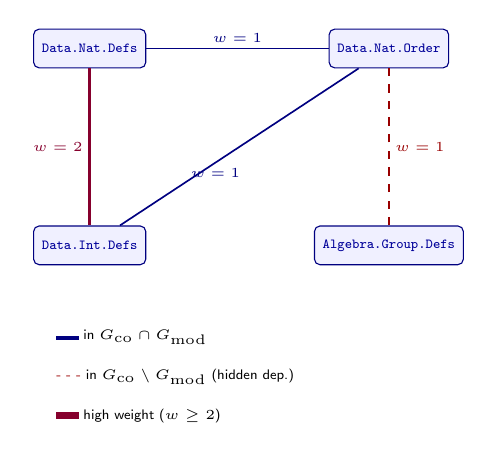
\begin{tikzpicture}[
  every node/.style={font=\scriptsize, inner sep=2pt},
  mod/.style={rounded corners=2pt, draw=blue!50!black, fill=blue!6,
    font=\tiny\ttfamily, text=blue!60!black, inner sep=3pt, minimum height=14pt},
  coedge/.style={-, blue!50!black, semithick},
  strongedge/.style={-, purple!70!black, very thick},
  hiddenedge/.style={-, red!60!black, semithick, dashed},
]
  % Nodes
  \node[mod] (natd) at (0, 2.5) {Data.Nat.Defs};
  \node[mod] (nato) at (3.8, 2.5) {Data.Nat.Order};
  \node[mod] (intd) at (0, 0) {Data.Int.Defs};
  \node[mod] (grpd) at (3.8, 0) {Algebra.Group.Defs};
  % Edges with weights
  % Strong edge: co-modified 2 times
  \draw[strongedge] (natd) -- node[left, font=\tiny\sffamily, text=purple!70!black] {$w=2$} (intd);
  % Normal edges: co-modified 1 time, also in G_module
  \draw[coedge] (natd) -- node[above, font=\tiny\sffamily, text=blue!50!black] {$w=1$} (nato);
  \draw[coedge] (intd) -- node[below, font=\tiny\sffamily, text=blue!50!black, pos=0.4] {$w=1$} (nato);
  % Hidden dependency: co-modified but NOT in G_module
  \draw[hiddenedge] (grpd) -- node[right, font=\tiny\sffamily, text=red!60!black] {$w=1$} (nato);
  % Legend
  \node[font=\tiny\sffamily, anchor=north west] at (-0.5, -1.0)
    {\textcolor{blue!50!black}{\rule{8pt}{1.5pt}} in $G_{\mathrm{co}} \cap G_{\mathrm{mod}}$};
  \node[font=\tiny\sffamily, anchor=north west] at (-0.5, -1.5)
    {\textcolor{red!60!black}{- - -} in $G_{\mathrm{co}} \setminus G_{\mathrm{mod}}$ (hidden dep.)};
  \node[font=\tiny\sffamily, anchor=north west] at (-0.5, -2.0)
    {\textcolor{purple!70!black}{\rule{8pt}{2.5pt}} high weight ($w \ge 2$)};
\end{tikzpicture}
\caption{$G_{\mathrm{co}}$: edge weight = number of PRs co-modifying both modules. The \textcolor{red!60!black}{dashed edge} has no import in $G_{\mathrm{mod}}$---a hidden dependency.}
\label{fig:co-edit-graph}
\end{subfigure}
\caption{Co-modification graph (Definition~\ref{def:co-edit-graph}). (a)~Three merged PRs and the files each touches. (b)~The resulting weighted undirected graph $G_{\mathrm{co}}$: \textcolor{blue!50!black}{solid} edges exist in both $G_{\mathrm{co}}$ and $G_{\mathrm{mod}}$ (structural + logical coupling); the \textcolor{red!60!black}{dashed} edge between \module{Algebra.Group.Defs} and \module{Data.Nat.Order} appears only in $G_{\mathrm{co}}$, revealing a hidden dependency invisible to the import graph. The \textcolor{purple!70!black}{thick} edge ($w=2$) indicates a stronger coupling. All names have the \module{Mathlib.}\ prefix removed.}
\label{fig:co-modification}
\end{figure}

This graph captures traces of \emph{human organizational process} from a data source entirely independent of Lean's compilation model: the Git history. Comparing $G_{\mathrm{co}}$ with $G_{\mathrm{module}}$ tests whether structural coupling predicts logical coupling. Module pairs with high co-modification weight but no direct import edge reveal hidden dependencies---candidates for refactoring or explicit import addition. Conversely, direct import edges with zero co-modification suggest stable, well-encapsulated interfaces.

\paragraph{Planned analyses.}
Extract $G_{\mathrm{co}}$ from the \module{Mathlib} Git log (approximately ${\sim}20{,}000$ merged PRs as of February 2026). Compute the overlap between high-weight edges in $G_{\mathrm{co}}$ and edges in $G_{\mathrm{module}}$. Identify module pairs with high logical coupling but no structural coupling.

\emph{This data can be extracted directly from the Git history using standard tools (no metaprogramming access required) and is deferred to future work.}

\subsubsection{Declaration Metadata as Node Attributes}
\label{sec:decl-metadata}

Beyond graph topology, declarations carry rich metadata that can serve as node-level attributes, enabling correlation analyses between structural position and declaration properties.

\begin{definition}[Declaration attributes]\label{def:decl-attributes}
The \emph{attribute function} $\alpha : \mathcal{D} \to \mathcal{P}(\mathcal{A})$ maps each declaration to its set of Lean attributes, where $\mathcal{A} = \{\texttt{simp},\, \texttt{ext},\, \texttt{to\_additive},\, \texttt{instance},\, \texttt{reducible},\, \texttt{inline},\, \ldots\}$. In particular:
\begin{itemize}
  \item The \emph{proof complexity} $\kappa(d) = |\{\text{Expr nodes in } d.\pi\}|$ measures proof term size.
  \item The \emph{universe polymorphism degree} $\upsilon(d) = |\text{universe parameters of } d|$.
  \item Two declarations satisfy $d_1 \sim_{\mathrm{add}} d_2$ when $\texttt{to\_additive} \in \alpha(d_1)$ and $d_2$ is the generated additive counterpart. The \emph{flattening ratio} $\phi = |\{d : \texttt{to\_additive} \in \alpha(d)\}| / |\mathcal{D}|$ quantifies the fraction of the library that exists as mirrored multiplicative/additive pairs.
\end{itemize}
\end{definition}

\begin{figure}[!htb]
\centering
\begin{subfigure}[t]{0.46\textwidth}
\centering
\vspace{0pt}
\raggedright\scriptsize\ttfamily
@[simp] \textbf{theorem} \textcolor{red!70!black}{mul\_one}\\
\hspace{1em}[Monoid $\alpha$] (a : $\alpha$) : a * 1 = a\\[6pt]
@[to\_additive] \textbf{theorem} \textcolor{red!70!black}{mul\_comm}\\
\hspace{1em}[CommMonoid $\alpha$] (a b : $\alpha$) : a * b = b * a\\[4pt]
\hspace{1em}\textnormal{\sffamily\tiny\textcolor{gray!50}{%
generates \decl{add\_comm} automatically}}\\[6pt]
@[simp, ext] \textbf{theorem} \textcolor{red!70!black}{Prod.mk.eta}\\
\hspace{1em}: (p.1, p.2) = p\\[10pt]
\textnormal{\sffamily Extracted metadata per node:}\\[2pt]
\hspace{1em}\textnormal{\sffamily\tiny%
$\alpha(d)$: attribute set \{simp, ext, \ldots\}}\\
\hspace{1em}\textnormal{\sffamily\tiny%
$\kappa(d)$: proof term size (Expr node count)}\\
\hspace{1em}\textnormal{\sffamily\tiny%
$\upsilon(d)$: universe polymorphism degree}
\caption{Declarations with Lean attributes and the metadata extracted from each.}
\label{fig:attr-source}
\end{subfigure}%
\hfill
\begin{subfigure}[t]{0.50\textwidth}
\centering
\vspace{0pt}
\begin{tikzpicture}[
  every node/.style={font=\scriptsize, inner sep=2pt},
  dot/.style={circle, fill=red!70!black, minimum size=4pt, inner sep=0pt},
  depedge/.style={->, >=Stealth, gray!50, semithick},
  tag/.style={rounded corners=1.5pt, font=\tiny\sffamily, inner sep=1.5pt},
  simptag/.style={tag, fill=teal!15, text=teal!70!black, draw=teal!40},
  exttag/.style={tag, fill=violet!15, text=violet!70!black, draw=violet!40},
  toaddtag/.style={tag, fill=orange!15, text=orange!70!black, draw=orange!40},
  mirror/.style={<->, >=Stealth, orange!60!black, semithick, dashed},
  meta/.style={font=\tiny\sffamily, text=gray!60},
]
  % Node: mul_one
  \node[dot, label={[font=\tiny\ttfamily, red!70!black]left:mul\_one}]
    (mo) at (0, 3.2) {};
  \node[simptag, anchor=west] at (0.25, 3.2) {simp};
  \node[meta, anchor=west] at (0.25, 2.8) {$\kappa=12$\enspace$\upsilon=1$};
  % Node: mul_comm
  \node[dot, label={[font=\tiny\ttfamily, red!70!black]left:mul\_comm}]
    (mc) at (0, 1.6) {};
  \node[toaddtag, anchor=north] at (0, 1.1) {to\_additive};
  \node[meta, anchor=west] at (0.25, 0.7) {$\kappa=34$\enspace$\upsilon=1$};
  % Node: add_comm (mirror)
  \node[dot, fill=orange!50!red, label={[font=\tiny\ttfamily, orange!60!black]right:add\_comm}]
    (ac) at (4.0, 1.6) {};
  \node[meta, anchor=west] at (4.25, 1.2) {$\kappa=34$\enspace$\upsilon=1$};
  % Node: Prod.mk.eta
  \node[dot, label={[font=\tiny\ttfamily, red!70!black]left:Prod.mk.eta}]
    (pe) at (0, -0.4) {};
  \node[simptag, anchor=west] at (0.25, -0.4) {simp};
  \node[exttag, anchor=west] at (1.05, -0.4) {ext};
  \node[meta, anchor=west] at (0.25, -0.85) {$\kappa=8$\enspace$\upsilon=2$};
  % Mirror edge (to_additive)
  \draw[mirror] (mc) -- node[above, font=\tiny\sffamily, text=orange!60!black] {$\sim_{\mathrm{add}}$} (ac);
  % Dependency edges (faint)
  \draw[depedge] (mo) -- (mc);
  \draw[depedge] (mc) -- (pe);
\end{tikzpicture}
\caption{Nodes of $G_{\mathrm{thm}}$ enriched with attribute tags, proof complexity~$\kappa$, and universe degree~$\upsilon$. The \textcolor{orange!60!black}{dashed} arrow marks a \texttt{to\_additive} mirror pair.}
\label{fig:attr-graph}
\end{subfigure}
\caption{Declaration metadata as node attributes (Definition~\ref{def:decl-attributes}). (a)~Lean source with attribute annotations. (b)~The declaration graph enriched with per-node metadata: colored tags indicate attributes ($\textcolor{teal!70!black}{\texttt{simp}}$, $\textcolor{violet!70!black}{\texttt{ext}}$, $\textcolor{orange!70!black}{\texttt{to\_additive}}$); $\kappa$ and $\upsilon$ are numeric features. The \textcolor{orange!60!black}{dashed} bidirectional arrow marks the automatically generated additive mirror \decl{add\_comm} $\sim_{\mathrm{add}}$ \decl{mul\_comm}.}
\label{fig:decl-attributes}
\end{figure}

These attributes bridge the two dimensions of our framework. Proof complexity~$\kappa$ and tactic usage characterize the \emph{process} layer (how theorems are proved), while $\upsilon$ and the \texttt{to\_additive} equivalence characterize \emph{tool-mediated structure}---features arising from Lean's type system and metaprogramming infrastructure rather than mathematical content. In particular, computing~$\phi$ would convert our qualitative observation about semantic flattening (\S\ref{sec:thm-vs-lemma}) into a precise count of automatically generated mirrors.

\paragraph{Definitional unfolding depth.}
Lean's type checker relies on \emph{definitional equality}: to verify that two types match, the kernel may need to unfold a chain of definitions. The \emph{unfolding depth} $\delta(d)$ counts the maximum number of definition expansions the kernel performs during type-checking of~$d$. This quantity is invisible in the explicit dependency graph $G_{\mathrm{thm}}$---it does not appear in $\mathrm{refs}(d.\pi)$---yet it constitutes a form of \emph{implicit coupling}: declarations with high~$\delta$ are brittle, because changes to any definition along the unfolding chain can break type-checking even if the explicit premise set is unchanged. The distribution of~$\delta$ across $\mathcal{D}$ measures the kernel's hidden workload, complementing the explicit dependency structure captured by $G_{\mathrm{thm}}$.

\paragraph{Planned analyses.}
Correlate $\kappa(d)$ with topological depth $\mathrm{depth}(d)$ and in-degree $\deg^{-}(d)$. Test whether universe-polymorphic declarations ($\upsilon(d) \ge 1$) have systematically higher in-degree. Precisely count \texttt{to\_additive} mirrors to quantify semantic flattening. Compute tactic usage distributions per top-level namespace and measure proof methodology variation across mathematical domains via Jensen--Shannon divergence. Correlate $\delta(d)$ with compilation time to test whether unfolding depth is a significant contributor to build bottlenecks.

\emph{Empirical analysis requires metaprogramming access to Lean's \texttt{Environment} API (for attributes, proof term sizes, universe parameters, and kernel-level unfolding traces) and is deferred to future work.}

\subsubsection{Temporal Graph Sequences}
\label{sec:temporal-graphs}

All analyses in this paper are computed from a single snapshot. A longitudinal extension would test whether the structural properties we observe are stable invariants of mathematical content or transient features of a particular development phase.

\begin{definition}[Temporal graph sequence]\label{def:temporal-sequence}
Let $\{c_1, c_2, \ldots, c_T\}$ be a sequence of $T$ historical \module{Mathlib} commits. Each commit $c_t$ yields an environment $\mathcal{E}_t$ and corresponding graphs $G_{\mathrm{thm}}^{(t)} = (\mathcal{D}_t, E_t)$ and $G_{\mathrm{mod}}^{(t)} = (\mathcal{M}_t, F_t)$. Define:
\begin{itemize}
  \item \emph{Growth indicators}: $|\mathcal{D}_t|$, $|\mathcal{M}_t|$, and edge density $|E_t| / |\mathcal{D}_t|$.
  \item \emph{Structural stability}: community persistence $\mathrm{NMI}(\mathcal{L}^{(t)}, \mathcal{L}^{(t+1)})$, hub turnover (rank correlation of in-degree rankings between consecutive snapshots), and redundancy trend $r(G_{\mathrm{mod}}^{(t)})$ over time.
  \item \emph{Structural events}: discontinuities in the time series coinciding with known events (e.g., the Lean~3$\to$4 port via Mathport, 2023; the module system introduction, November 2025).
\end{itemize}
\end{definition}

\begin{figure}[!htb]
\centering
\begin{subfigure}[t]{0.38\textwidth}
\centering
\vspace{0pt}
\raggedright\scriptsize
\textsf{\bfseries Timeline of snapshots}\\[6pt]
\begin{tikzpicture}[
  every node/.style={font=\tiny\sffamily},
  dot/.style={circle, fill=blue!60!black, minimum size=3pt, inner sep=0pt},
  event/.style={font=\tiny\sffamily\itshape, text=red!60!black},
]
  % Timeline
  \draw[->, >=Stealth, gray!60, thick] (0, 0) -- (0, -5.2);
  \node[font=\tiny\sffamily, gray!50, anchor=east] at (-0.15, 0) {$t$};
  % Snapshots
  \node[dot] (c1) at (0, -0.3) {};
  \node[anchor=west] at (0.2, -0.3) {$c_1$: Jan 2023};
  \node[dot] (c2) at (0, -1.2) {};
  \node[anchor=west] at (0.2, -1.2) {$c_2$: Jul 2023};
  \node[event, anchor=west] at (0.2, -1.55) {Lean 3$\to$4 port};
  \node[dot] (c3) at (0, -2.4) {};
  \node[anchor=west] at (0.2, -2.4) {$c_3$: Jan 2024};
  \node[dot] (c4) at (0, -3.3) {};
  \node[anchor=west] at (0.2, -3.3) {$c_4$: Jan 2025};
  \node[dot] (c5) at (0, -4.2) {};
  \node[anchor=west] at (0.2, -4.2) {$c_5$: Nov 2025};
  \node[event, anchor=west] at (0.2, -4.55) {module system};
  \node[dot, fill=orange!80!red] (c6) at (0, -5.0) {};
  \node[anchor=west, text=orange!80!red] at (0.2, -5.0) {$c_T$: Feb 2026 (this paper)};
\end{tikzpicture}
\caption{Monthly snapshots $\{c_1, \ldots, c_T\}$ with structural events marked.}
\label{fig:temporal-timeline}
\end{subfigure}%
\hfill
\begin{subfigure}[t]{0.58\textwidth}
\centering
\vspace{0pt}
\begin{tikzpicture}[
  every node/.style={font=\scriptsize, inner sep=2pt},
  mod/.style={circle, fill=blue!60!black, minimum size=2.5pt, inner sep=0pt},
  edge/.style={-, blue!30!black, semithick, opacity=0.5},
  frame/.style={rounded corners=3pt, draw=gray!40, fill=gray!3, inner sep=4pt},
]
  % Graph at t=1 (small)
  \node[frame, minimum width=50pt, minimum height=40pt] (f1) at (0, -0.5) {};
  \node[font=\tiny\sffamily, gray!60, above=0pt of f1] {$G^{(c_1)}$};
  \node[mod] (a1) at (-0.4, -0.2) {};
  \node[mod] (b1) at (0.3, -0.1) {};
  \node[mod] (c1n) at (-0.1, -0.7) {};
  \node[mod] (d1) at (0.5, -0.8) {};
  \draw[edge] (a1) -- (b1);
  \draw[edge] (b1) -- (c1n);
  \draw[edge] (c1n) -- (d1);
  % Growth indicators
  \node[font=\tiny\sffamily, text=gray!50, below=2pt of f1] {$|\mathcal{D}|{=}50\text{k}$};
  % Graph at t=3 (medium)
  \node[frame, minimum width=55pt, minimum height=45pt] (f3) at (2.3, -0.5) {};
  \node[font=\tiny\sffamily, gray!60, above=0pt of f3] {$G^{(c_3)}$};
  \node[mod] (a3) at (1.8, -0.1) {};
  \node[mod] (b3) at (2.5, 0.0) {};
  \node[mod] (c3n) at (2.0, -0.5) {};
  \node[mod] (d3) at (2.7, -0.4) {};
  \node[mod] (e3) at (2.3, -0.9) {};
  \node[mod] (f3n) at (1.9, -0.9) {};
  \draw[edge] (a3) -- (b3);
  \draw[edge] (a3) -- (c3n);
  \draw[edge] (b3) -- (d3);
  \draw[edge] (c3n) -- (e3);
  \draw[edge] (d3) -- (e3);
  \draw[edge] (c3n) -- (f3n);
  \node[font=\tiny\sffamily, text=gray!50, below=2pt of f3] {$|\mathcal{D}|{=}150\text{k}$};
  % Graph at t=T (large, current)
  \node[frame, minimum width=62pt, minimum height=50pt, draw=orange!60!red] (fT) at (4.8, -0.5) {};
  \node[font=\tiny\sffamily, orange!80!red, above=0pt of fT] {$G^{(c_T)}$};
  \node[mod, fill=orange!80!red] (aT) at (4.3, 0.0) {};
  \node[mod, fill=orange!80!red] (bT) at (5.0, 0.1) {};
  \node[mod, fill=orange!80!red] (cT) at (4.5, -0.3) {};
  \node[mod, fill=orange!80!red] (dT) at (5.2, -0.3) {};
  \node[mod, fill=orange!80!red] (eT) at (4.3, -0.7) {};
  \node[mod, fill=orange!80!red] (fT2) at (4.8, -1.0) {};
  \node[mod, fill=orange!80!red] (gT) at (5.3, -0.7) {};
  \node[mod, fill=orange!80!red] (hT) at (4.6, -0.5) {};
  \draw[-, orange!40!red, semithick, opacity=0.5] (aT) -- (bT);
  \draw[-, orange!40!red, semithick, opacity=0.5] (aT) -- (cT);
  \draw[-, orange!40!red, semithick, opacity=0.5] (bT) -- (dT);
  \draw[-, orange!40!red, semithick, opacity=0.5] (cT) -- (eT);
  \draw[-, orange!40!red, semithick, opacity=0.5] (dT) -- (gT);
  \draw[-, orange!40!red, semithick, opacity=0.5] (eT) -- (fT2);
  \draw[-, orange!40!red, semithick, opacity=0.5] (hT) -- (fT2);
  \draw[-, orange!40!red, semithick, opacity=0.5] (cT) -- (hT);
  \draw[-, orange!40!red, semithick, opacity=0.5] (gT) -- (fT2);
  \node[font=\tiny\sffamily, text=orange!80!red, below=2pt of fT] {$|\mathcal{D}|{=}318\text{k}$};
  % Growth arrows
  \draw[->, >=Stealth, gray!40, thick] (0.95, -0.5) -- (1.55, -0.5);
  \node[font=\tiny\sffamily, gray!40, above] at (1.25, -0.5) {$\cdots$};
  \draw[->, >=Stealth, gray!40, thick] (3.15, -0.5) -- (3.95, -0.5);
  \node[font=\tiny\sffamily, gray!40, above] at (3.55, -0.5) {$\cdots$};
  % Tracked metrics below
  \node[font=\tiny\sffamily, anchor=north west] at (-0.8, -2.0)
    {Track: $|\mathcal{D}_t|$, edge density, community NMI, hub turnover, redundancy $r(G_{\mathrm{mod}}^{(t)})$};
\end{tikzpicture}
\caption{Graph snapshots growing over time; structural metrics tracked across the sequence detect events and trends.}
\label{fig:temporal-graph}
\end{subfigure}
\caption{Temporal graph sequence (Definition~\ref{def:temporal-sequence}). (a)~Monthly snapshots of \module{Mathlib} commits, with two structural events: the Lean~3$\to$4 port (2023) and the module system introduction (November 2025). (b)~The declaration graph $G_{\mathrm{thm}}^{(t)}$ at three time points, growing from ${\sim}50$k to $318$k declarations. Tracking structural indicators across the sequence reveals whether properties like the $17.5\%$ redundancy rate are stable invariants or transient features of a particular development phase.}
\label{fig:temporal-sequence}
\end{figure}

The temporal dimension directly captures the \emph{process} of organizational restructuring. If \module{Mathlib}'s dependency structure is primarily determined by inherited mathematical logic, structural indicators should be stable under refactoring; if organizational process dominates, we expect significant structural change at refactoring events while mathematical content remains constant. The Lean~3$\to$4 port is a natural experiment: identical mathematical content, entirely rewritten proof infrastructure.

\paragraph{Planned analyses.}
Construct $G^{(t)}$ for monthly snapshots spanning the post-port era (2023--2026). Track growth indicators, structural stability, and redundancy trends. Test whether the $17.5\%$ redundancy rate and $0.107$ cohesion are increasing, stable, or approaching critical thresholds.

\emph{Longitudinal analysis requires running the extraction pipeline across multiple historical commits and is deferred to future work.}
